	\chapter{Computer Vision Prework}

	\section{Emergence of Convolution}
	\subsection{Feature Extraction}
	\begin{bulletedlist}
		\item What is a feature (in an image)?
		\begin{bulletedlist}
			\item Features are various forms of information that can be gained from an image.  For example: Fig 1 has various features, such as shape, size, color, edges, and background.  These features play a crucial role in helping perform several tasks in computer vision like image classification, object detection, scene detection, etc.
		\end{bulletedlist}
		\item The features required by each task in computer vision are completely task-dependent, and each task might not require all the features available in an image.  For example, we can still identify that the right side of \figurename~\ref{fig:imagefeatureextraction} is an image of a duck (even though it is harder to do than for the left) without necessarily knowing the color or background of the image, but only from looking at the edges, the presence of water and the shape of the bird inside the image.
		\item Hence, we need methods to extract just the essential information contained in images and ignore the rest depending on different tasks. This step is called feature extraction.
		\item The features we obtain from feature extraction are crucial in enhancing the model's performance.
		\item Feature extraction methods help in converting images to certain feature vectors of fixed sizes.
		\item Some of the most important feature extraction techniques to have been used with images are:
		\begin{bulletedlist}
			\item HOG (Histogram of Oriented Gradients)
			\item SIFT (Scale Invariant Feature Transform)
			\item Convolution Operations
		\end{bulletedlist}
	\end{bulletedlist}

	\begin{figure}[h]
		\centering
		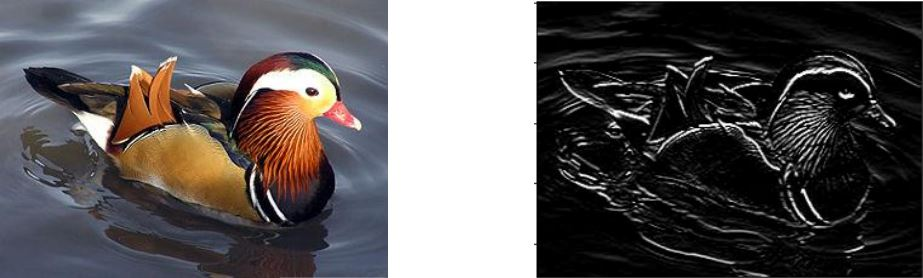
\includegraphics[height=1.5in]{imagefeatureextraction}
		\caption[Feature extraction]{Feature extraction.}
		\label{fig:imagefeatureextraction}
	\end{figure}

	\subsection{Conventional Feature Extraction Techniques}
The two most historically-important, manual feature extraction techniques have been:
	\begin{bulletedlist}
		\item HOG (Histogram of Oriented Gradients)
		\item SIFT (Scale Invariant Feature Transform)
	\end{bulletedlist}

	\begin{table}
        \centering
        \caption[HOG versus SIFT feature extraction]{HOG versus SIFT feature extraction.}
        \label{tab:hogversussift}
		\begin{tabular}{|p{0.5\textwidth-2\tabcolsep}|p{0.5\textwidth-2\tabcolsep}|} \hline
				\tablecolumnheadervlinesone{HOG} & \tablecolumnheadervlinestwo{SIFT} \\ \hline
				HOG mainly focuses on the structure and shape of an object. &
	            In SIFT, image content is converted into local feature coordinates. \\ \hline
				Image manipulation effects HOG.  For example, scaling will reduce gradient. &
				SIFT is not effected rotation, scaling, or other image manipulations. \\ \hline
				HOG is different from only detecting edges, as it also identifies the magnitude and direction of edges in the image. &
	            SIFT assists in locating the local features of an image, often known as image keypoints. \\ \hline
				HOG calculates the magnitude and direction of edges in each region. The Orientation is the direction and the Gradient is the magnitude of the pixel values of the image. &
				The key points obtained from SIFT can be utilised for picture matching, object detection, scene detection, and other computer vision applications. \\ \hline
				\adjustbox{center}{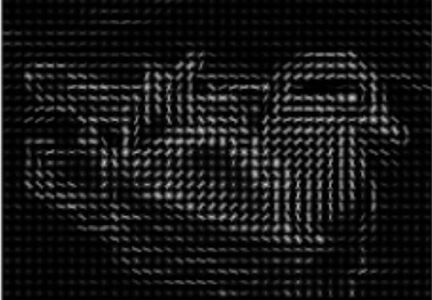
\includegraphics[height=1.5in]{hogfeaturedetection}} &
				\adjustbox{center}{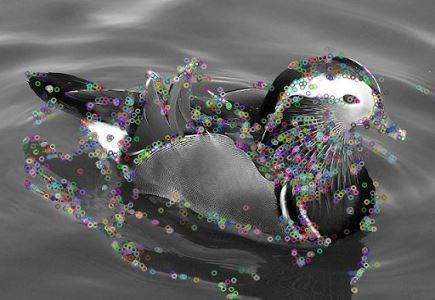
\includegraphics[height=1.5in]{siftfeaturedetection}} \\ \hline
		\end{tabular}
	\end{table}

	\subsection{Disadvantages of Conventional Feature Extraction Techniques}
	\begin{bulletedlist}
		\item Why was SIFT preferred over HOG?
		\begin{bulletedlist}
			\item SIFT features, as opposed to HOG features, have the advantage of being unaffected by the image's size or orientation.
			\item SIFT has a better accuracy than HOG for detecting features in an image.
			\item HOG is not scale and rotation invariant, whereas SIFT shows those properties.
		\end{bulletedlist}
		\item However, both SIFT and HOG showed certain disadvantages in the efforts to apply them as general feature extraction techniques for all images:
		\begin{bulletedlist}
			\item Both SIFT and HOG are quite slow and computationally expensive.
			\item They are also somewhat mathematically complex in their working.
			\item In addition, HOG does not work well with lighting changes and blurring in the images.
		\end{bulletedlist}
	\end{bulletedlist}

	\subsection{Convolution Over SIFT and HOG}

	\begin{bulletedlist}
		\item Convolution is a specialized linear operation on an image, that represents an efficient way of extracting image features and reducing the dimensions of an image.
		\item Convolution consists of a set of filters called convolution layers, that perform convolution operations on images.
		\item We use multiple filters to perform convolution operations on an image, and try to extract various kinds of features (pertaining to each kind of filter) from a single image.
		\item For example, let's assume that we need to use convolutions to extract features from an image of a brick wall (shown in \figurename~\ref{fig:convolutionbrickwall}).  We may be interested in each of the following feature extraction tasks:
		\begin{bulletedlist}
			\item to extract all the vertical edges from the image
			\item to extract all the horizontal edges from the image
			\item to blur/sharpen the image
			\item To highlight/focus on certain places of image
		\end{bulletedlist}
		\item As seen from the below example in \figurename~\ref{fig:convolutionbrickwalledgedetection}, convolution filters can help us achieve any of the feature extraction tasks we may require for our images.
	\end{bulletedlist}

	\begin{figure}[h]
		\centering
		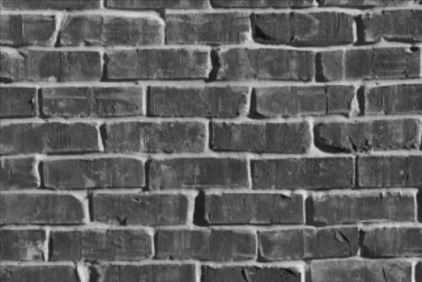
\includegraphics[height=1.25in]{convolutionbrickwall}
		\caption[Image of a brick used for convolution example]{Image of a brick used for convolution example.}
		\label{fig:convolutionbrickwall}
	\end{figure}

	\begin{figure}[h]
		\centering
		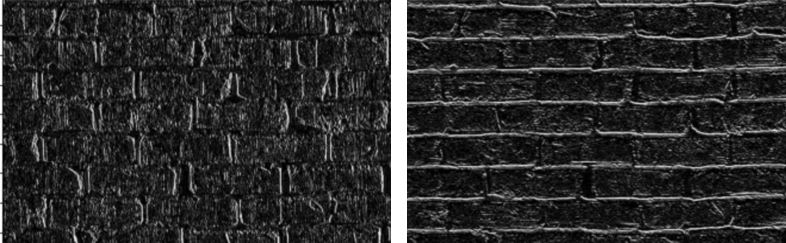
\includegraphics[height=1.25in]{convolutionbrickwalledgedetection}
		\caption[Convolution vertical and horizontal edge detection]{Image of brick wall with vertical edge detection (left) and horizontal edge detection (right).}
		\label{fig:convolutionbrickwalledgedetection}
	\end{figure}

	\subsection{Convolution over SIFT and HOG}

Why is Convolution better than SIFT and HOG?
	\begin{bulletedlist}
		\item Convolutional feature detectors are highly trainable and adaptable, allowing them to achieve higher accuracy levels in comparison to SIFT and HOG for the task at hand.
		\item Convolutions excel at learning low-level features of an image in a much better way than SIFT and HOG, and they do so without the overhead of the hand-coded feature engineering which is usually required for SIFT and HOG.
		\item Apart from learning low-level features, hierarchical combinations of convolutions are quite effective in learning important high-level features as well.  Example: for images of human faces, convolutional layers would easily learn to understand more
complex shapes such as the eyes, the ears, the nose or the mouth.
		\item In 2012, AlexNet, a Convolutional Neural Network (CNN) architecture, based fundamentally on the principle of convolutional filters, handily won the famous ImageNet competition - outperforming the runner-up by over 10 percentage points.  Although convolutions were already known in literature from the work of Yann LeCun, this breakthrough is what drew attention from the whole technology industry to the power of convolutions in image feature extraction.
		\item It soon became clear to machine learning practitioners that hierarchical combinations of convolution filters achieved superior and far more generalizable results in image feature extraction than SIFT and HOG. This is the fundamental driver behind the emergence of convolutions as part of Convolutional Neural Networks (CNNs), which have become a staple in state-of-the-art deep learning models for computer vision over the last decade.
	\end{bulletedlist}



	\section{Edge Detection and Kernels}
	\subsection{Convolution and Edge Detection}
	\subsubsection{Edge Detection}
	\begin{bulletedlist}
		\item As we previously discussed, the Convolution operation is the fundamental building block of Convolutional Neural Networks.

		\item Let's try to understand how the Convolution process works, with the help of the Edge Detection concept that Convolution filters are able to perform.
		\item Mathematically in terms of pixel intensity values, edges are image regions where there is a sudden, sharp change in the brightness of the pixels. This can be observed by a large change in the pixel intensity values among neighboring pixels in some direction.
		\item Let us first convert the image in \figurename~\ref{fig:edgedetectioncross} into its gray scale version, so that we have a 2D matrix to work with for us to analyze the pixel intensity values of the image (\figurename~\ref{fig:convolutionbrickwalledgedetection}).
		\item The information about edges in images is usually preserved during gray scale conversion for most of the images we will work with, so we don't have to worry about color information loss for now.
		\item We observe that there is a clear gradient or change in pixel intensity values either side of the lines drawn inside this matrix. (Ex: 255 on one side and 116 and 61 on the other).
		\item These gradient lines also mirror the ``+'' shape of the edges of the image, so we know that they are a mathematical representation of what we visually perceive to be edges inside the image.
		\item This gradient of pixel intensity values is hence the mathematical meaning of an edge inside an image.
		\begin{bulletedlist}
			\item
		\end{bulletedlist}
	\end{bulletedlist}

	\begin{figure}[h]
		\centering
		
\includegraphics[height=0.85in]{edgedetectioncross}
		\caption[Edge detection step 1]{Edge detection step 1.}
		\label{fig:edgedetectioncross}
	\end{figure}
	\begin{figure}[h]
		\centering
		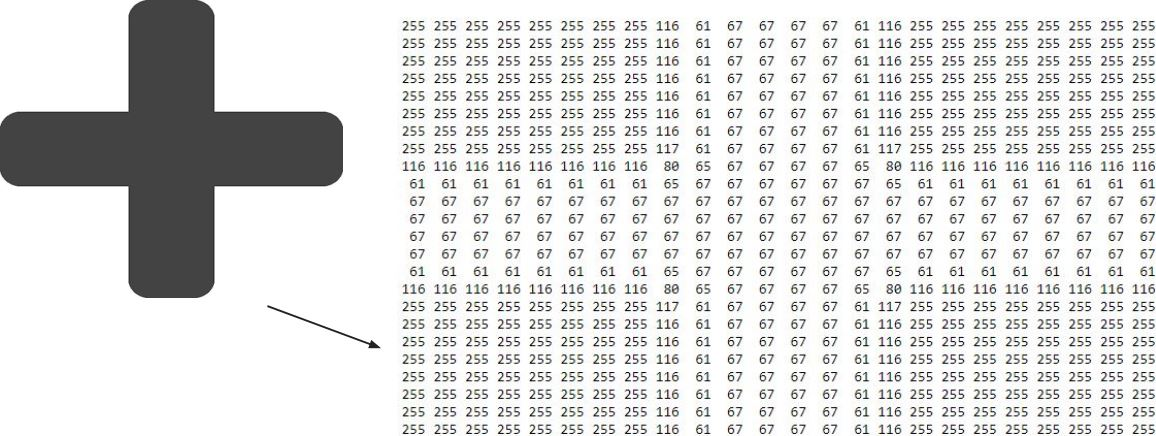
\includegraphics[height=1.25in]{edgedetectioncrossgrayscale}
		\caption[Edge detection step 2]{Edge detection step 2.}
		\label{fig:edgedetectioncrossgrayscale}
	\end{figure}
	\begin{figure}[h]
		\centering
		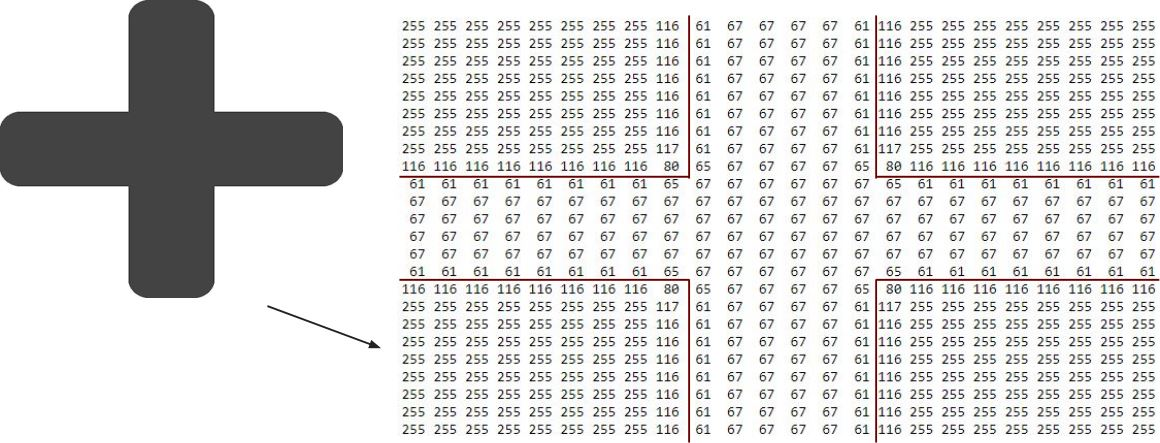
\includegraphics[height=1.25in]{edgedetectioncrossgrayscale2}
		\caption[Edge detection step 3]{Edge detection step 3.}
		\label{fig:edgedetectioncrossgrayscale2}
	\end{figure}

	\subsection{The importance of Edges}
	\begin{bulletedlist}
		\item So why are edges important?  Let's try to understand this with an example.
		\item In the left side of \figurename~\ref{fig:edgedetectioncar}, we have a gray scale image of a Ferrari 456 GT, a famous sports car from the nineties.
		\item On the right is another version of the same image, but with purely the edges of the image of the car on the left, and with very little information retained about the background.
		\item Can we still identify the presence of the car despite this loss of information?  Yes, we can!
		\item What this means, is that we can identify objects in an image based purely on the information about their edges, even by completely ignoring their background or other minute details of the image that are not important in detecting that object.
Therein lies the importance of edges in image prediction tasks.
		\item Edge detection is one of the primary tasks in object detection and object recognition.
		\item A lot of information about an image is found within its edges. So detecting edges and enhancing those areas should be our focus in image processing for the purpose of image classification tasks.
		\item One way to mathematically detect edges in an image is to perform convolution operations on a input image with a small array of numbers, also called a Filter / Kernel.
		\item The term Kernel refers to a 2D array, while the term Filter generally refers to multiple kernels stacked
together, to operate across a whole N-dimensional array. However the terms Kernel and Filter are often
used interchangeably across the industry.
		\item There are essentially three steps involved in the convolution operation:
		\begin{numberedlist}
			\item Taking in the Input Image as a Pixelmap.
			\item Applying a Filter / Kernel on the Input Image Pixelmap.
			\item Obtaining the Output Feature map
		\end{numberedlist}
	\end{bulletedlist}

	\begin{figure}[h]
		\centering
		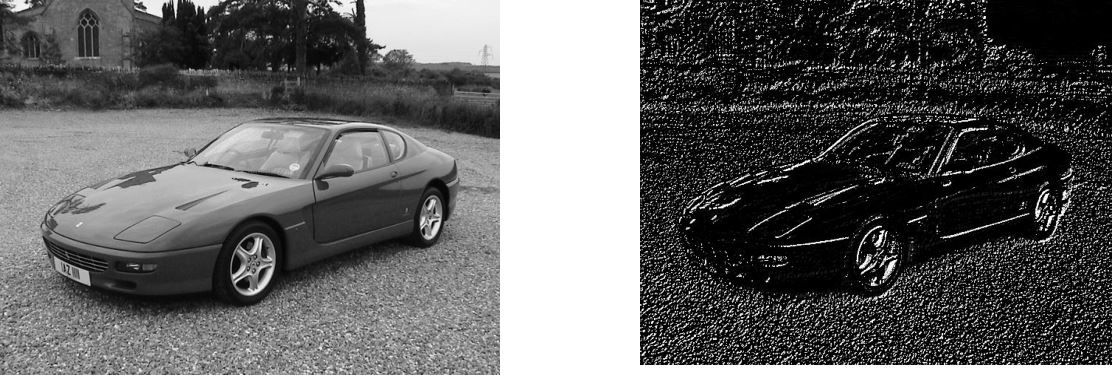
\includegraphics[height=1.5in]{edgedetectioncar}
		\caption[Edge detection example]{Edge detection example.}
		\label{fig:edgedetectioncar}
	\end{figure}

	\subsection{How to Detect Edges}

	\begin{bulletedlist}
		\item \figurename~\ref{fig:convolutededgedetection} is a representation of this three-stage convolution process.
		\item In the process, an input image (taken in the form of its pixelmap) is convolved with a kernel or filter, 	in order to obtain an output feature map.
		\item The above filter containing 1s, 0s and -1s, is an example of a vertical edge detector, as the pattern of numbers in the filter is vertically consistent (top to bottom) and will hence likely detect vertical edges inside the image.
		\item Let us now try to understand the mathematical working of convolution kernels, in order to understand the intuition behind how kernel edge detectors work.
	\end{bulletedlist}

	\begin{figure}[h]
		\centering
		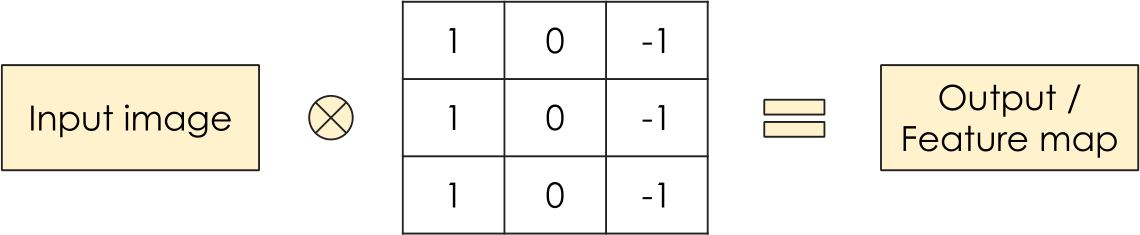
\includegraphics[height=0.7in]{convolutededgedetection}
		\caption{Image convoluted with a filter to produce a feature map.}
		\label{fig:convolutededgedetection}
	\end{figure}

	\begin{numberedlist}
		\item The filter is first superimposed over the first corresponding 3 x 3 region of the image, taking the products of the corresponding elements from the image and the filter, and then adding all these products to get a final sum.
		\item In other words, we take the sum of the element-wise products of the input region and the filter, to get the final number 510.
		\item The filter then slides over the input image array (with a default stride of 1), with a new sum of element-wise products being computed from the new region of the image over which the filter is now superimposed.
		\item This new sum of element-wise products again gives us the number 510, which goes into the second element of the output feature map.
		\item In the same way, the filter slides over the rest of the row in the input image array, and for each slide, the corresponding sum of element-wise products is computed and added to the relevant cell in the output feature map.
		\item In the same way, the filter slides over the rest of the row in the input image array, and for each slide, the corresponding sum of element-wise products is computed and added to the relevant cell in the output feature map.
		\item As seen above, with a 6 x 6 image and a 3 x 3 filter, we reach the end of the row after the 4th sliding position.
		\item Once the filter has completed the first row, the same sliding mechanism moves in the column direction to the next row. The same sliding of the filter is then carried out from the start to the end of the next row.
		\item The sum of element-wise products is computed in the same fashion, to give a new number 255, which goes into the first cell of the next row in the output.
		\item This sliding mechanism continues till the last row and last column, and the sum of element-wise products goes to the right cell in the output matrix.
		\item In general, for an n x n input image, and an f x f filter size, the output feature map will have dimensions of (n-f+1) x (n-f+1).
		\item That is how we have an output dimension of (6-3+1) x (6-3+1) or 4 x 4 here.
	\end{numberedlist}

	\begin{figure}[tbp]
		\begin{minipage}[t]{\textwidth}
			\begin{minipage}[t]{\textwidth}
				\centering
				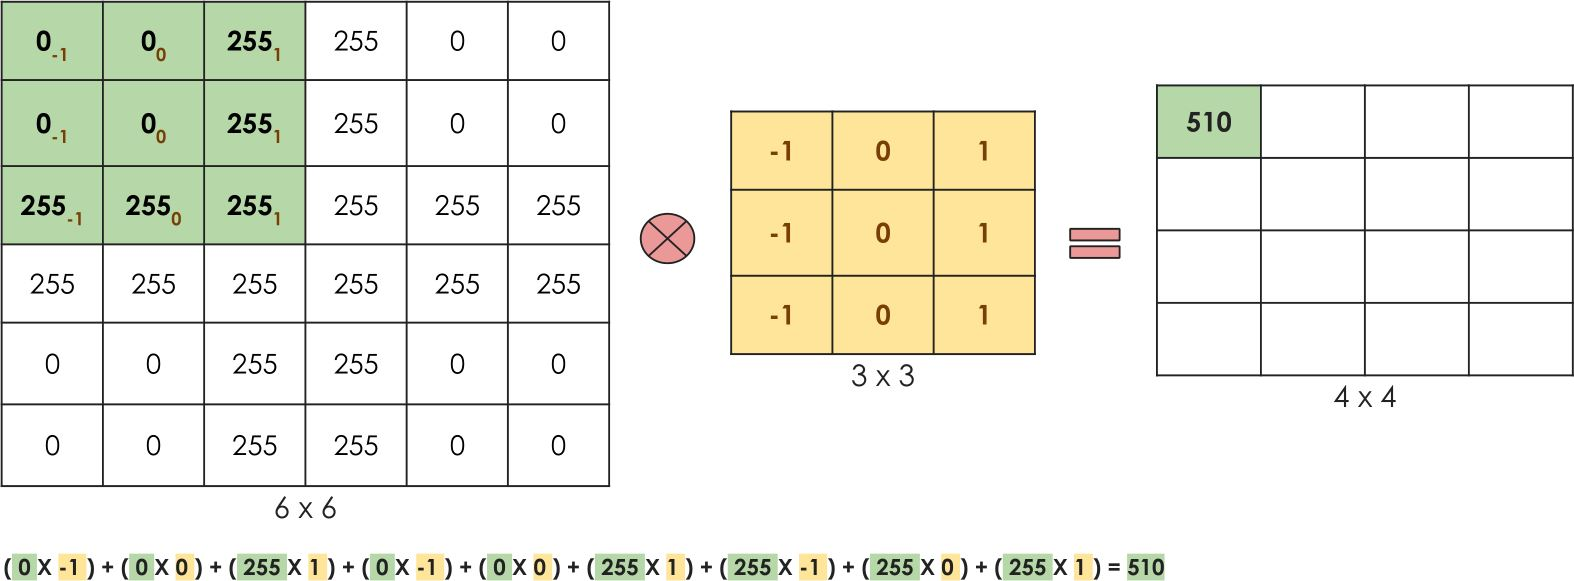
\includegraphics[height=1.5in]{convolutionoperationstep1}
				\subcaption{Step 1}
				\label{fig:convolutionoperationstep1}
			\end{minipage}
			\begin{minipage}[t]{\textwidth}
				\centering
				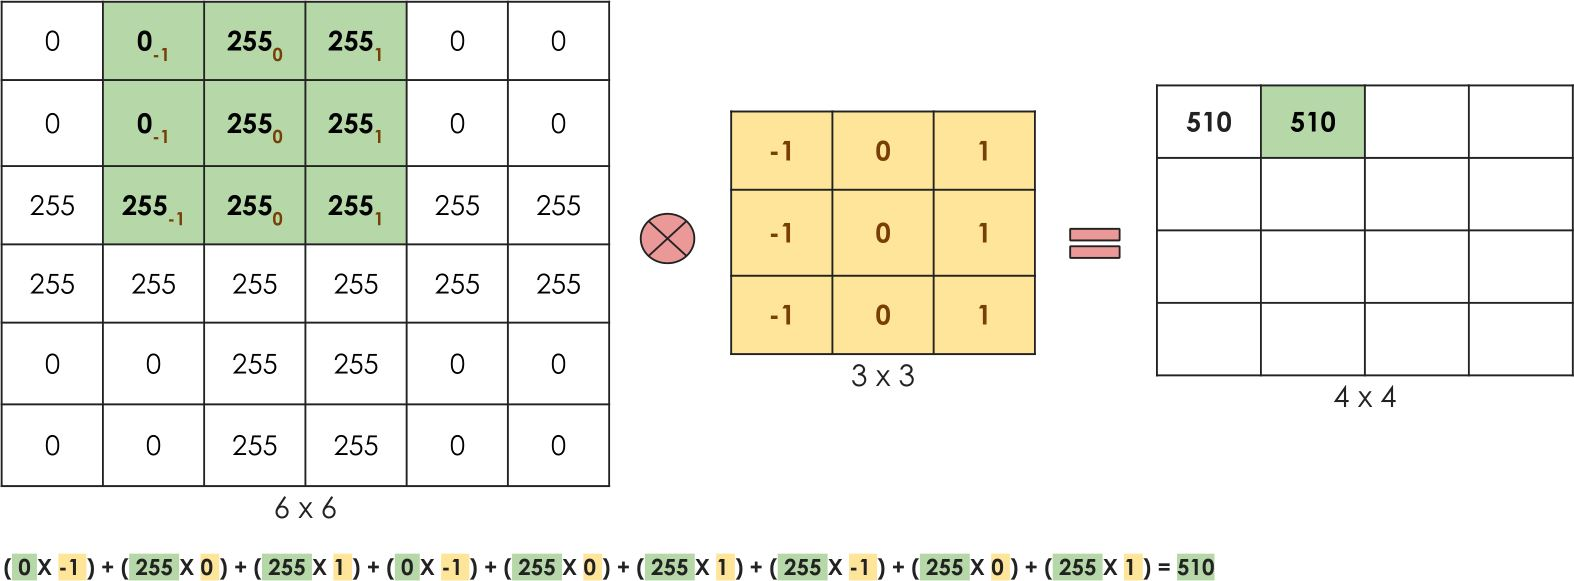
\includegraphics[height=1.5in]{convolutionoperationstep2}
				\subcaption{Step 2}
				\label{fig:convolutionoperationstep2}
			\end{minipage}
			\begin{minipage}[t]{\textwidth}
				\centering
				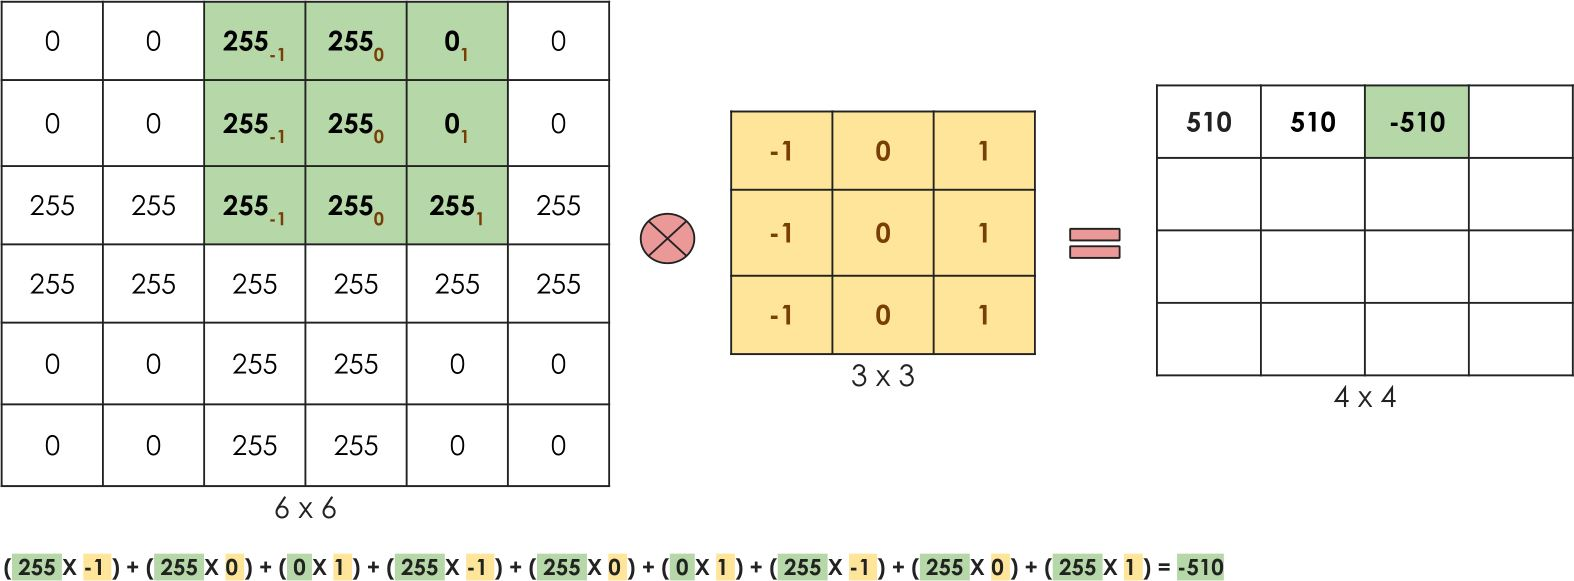
\includegraphics[height=1.5in]{convolutionoperationstep3}
				\subcaption{Step 3}
				\label{fig:convolutionoperationstep3}
			\end{minipage}
		\end{minipage}
		\caption{Edge detection steps, part 1.}
		\label{fig:convolutionoperationstepsa}
	\end{figure}

	\begin{figure}[tbp]
		\begin{minipage}[t]{\textwidth}
			\begin{minipage}[t]{\textwidth}
				\centering
				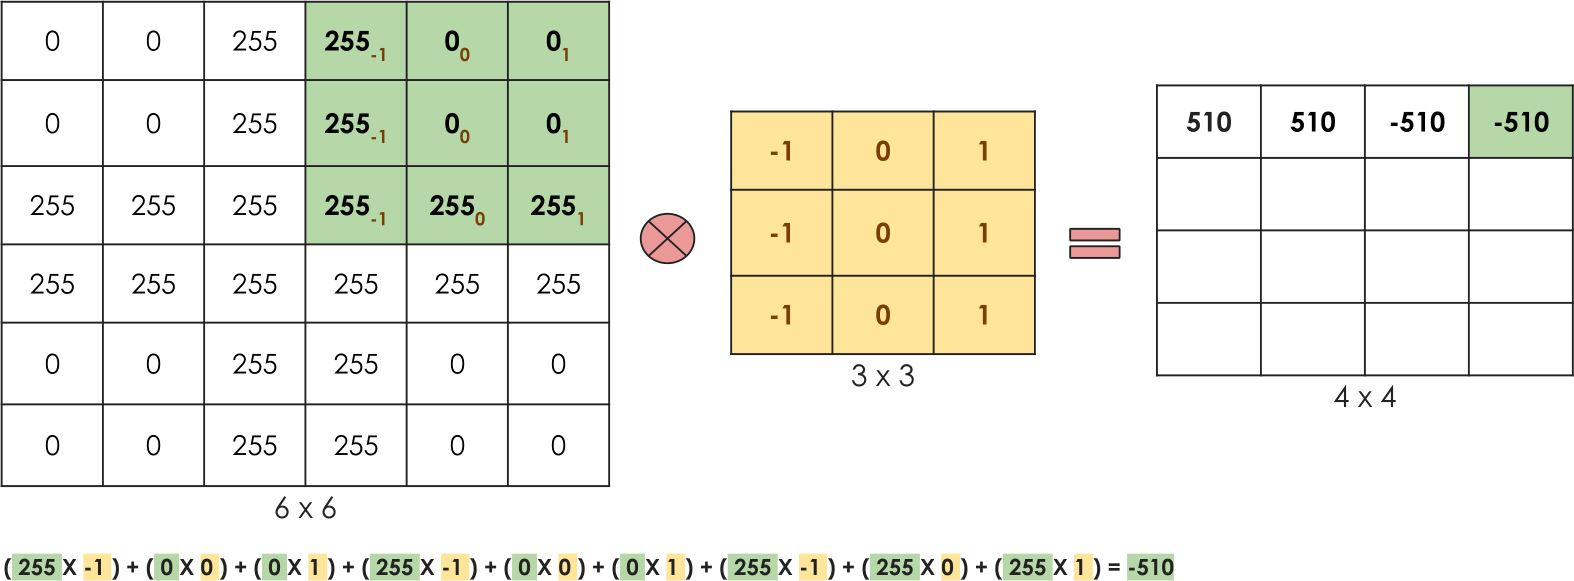
\includegraphics[height=1.5in]{convolutionoperationstep4}
				\subcaption{Step 4}
				\label{fig:convolutionoperationstep4}
			\end{minipage}
			\begin{minipage}[t]{\textwidth}
				\centering
				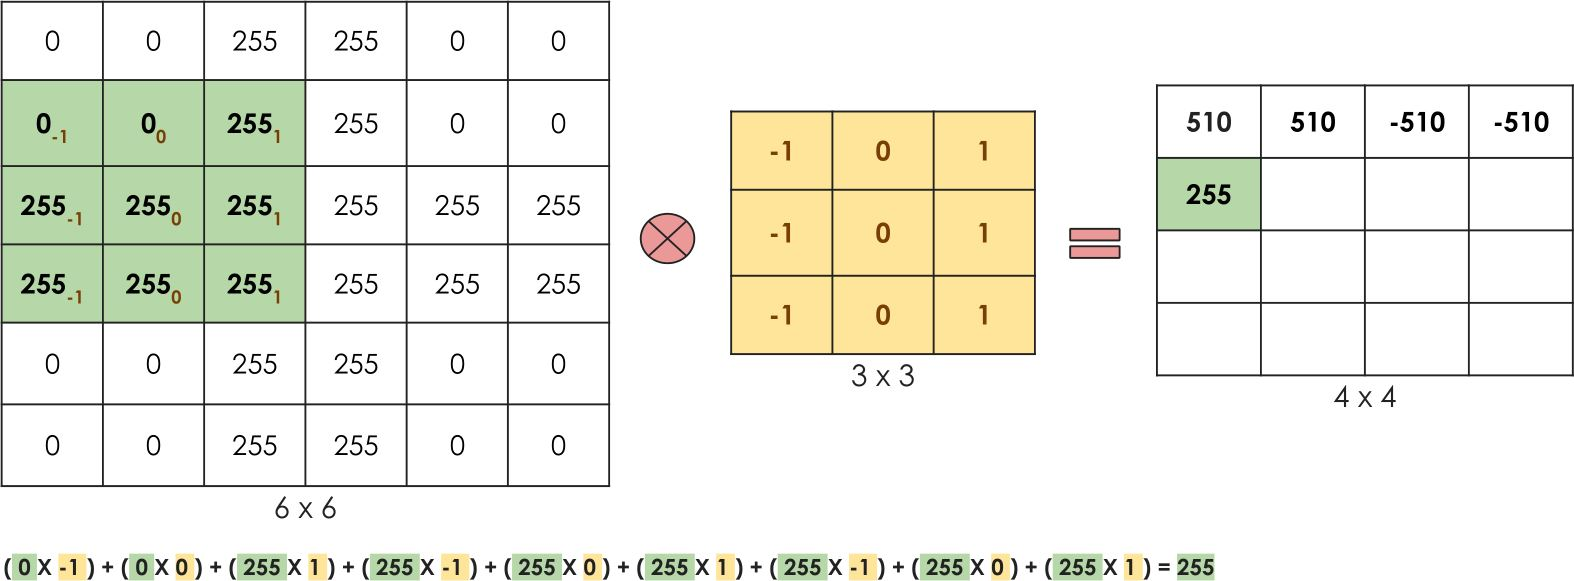
\includegraphics[height=1.5in]{convolutionoperationstep5}
				\subcaption{Step 5}
				\label{fig:convolutionoperationstep5}
			\end{minipage}
			\begin{minipage}[t]{\textwidth}
				\centering
				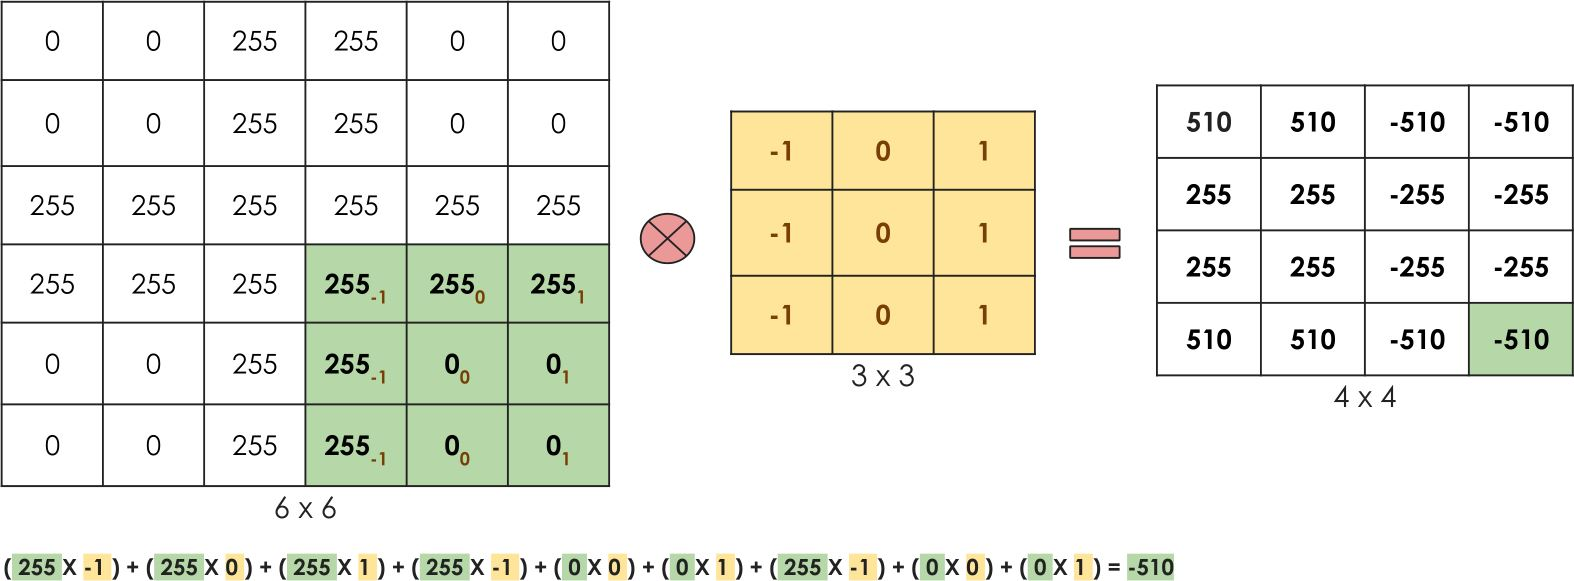
\includegraphics[height=1.5in]{convolutionoperationstep6}
				\subcaption{Step 6}
				\label{fig:convolutionoperationstep6}
			\end{minipage}
		\end{minipage}
		\caption{Edge detection steps, part 2.}
		\label{fig:convolutionoperationstepsb}
	\end{figure}

	\subsection{Intuition behind Convolutions}

	\begin{bulletedlist}
		\item Convolutions can be used for various kinds of feature extraction tasks, depending only on the pixel pattern of the filter.
		\item The convolution filter used in the previous example, for instance, has a vertical pattern of -1s, 0s and 1s.  It is also known in the industry as the Prewitt Filter.
		\item The above convolution filter would be considered a type of vertical edge detector, capable of identifying vertical edges in the image.
		\item The reason for this is due to the nature of the convolution operation, which uses a sum of element-wise products. The  implication of that is those regions of the image which have similar vertical patterns to those of the filter, get amplified in the element-wise product, and hence in the output matrix.
		\item In other words, convolution filters are adept at identifying those regions of the image which have pixel patterns that match the pixel pattern of the filter itself.
		\item That is why the above filter would be considered a type of vertical edge detector.  It has a vertical pattern of pixels (-1s, 0s and 1s) which represent a left-to-right increasing gradient.  Any regions in the input image that have a similar pattern to this would be identified by this filter, and amplified numerically with a higher output value for those regions.
		\item One other point of consideration is that filters with odd-valued dimensions (such as 3 x 3 Filters) are preferred, due to the presence of a central pixel.  The central pixel acts as a focus point and the filter is looking at the area surrounding the pixel.
	\end{bulletedlist}


	\subsection{Filters and Kernels}
	\begin{bulletedlist}
		\item Convolution filters can hence be used for various image manipulation tasks, such as edge detection, sharpening or blurring.
		\item As an example, let us discuss three convolution filters which have gained popularity over the years:
		\begin{bulletedlist}
			\item The Prewitt filter
			\item The Sobel filter
			\item The Laplacian filter
		\end{bulletedlist}
	\end{bulletedlist}

	\subsubsection{The Prewitt Filter}
	\begin{bulletedlist}
		\item The Prewitt filter (named after Judith M.S. Prewitt) has mostly been used in research for detecting horizontal and vertical edges in an image.
		\item This filter has three properties:
		\begin{bulletedlist}
			\item The sum of the elements in the filter is zero.
			\item The elements present in the filter should have opposite signs.
			\item The higher the magnitude of the positive and negative numbers, the higher the chances of detecting an edge.
		\end{bulletedlist}
		\item There are actually two variations of the filter, for detecting edges in both the horizontal and the vertical
directions.
	\end{bulletedlist}

	\begin{figure}[h]
		\centering
		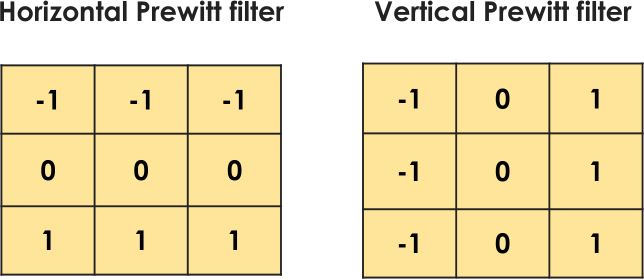
\includegraphics[height=1.0in]{prewittfilter}
		\caption[Prewitt filter]{Prewitt filter.}
		\label{fig:prewittfilter}
	\end{figure}
	\begin{figure}[h]
		\centering
		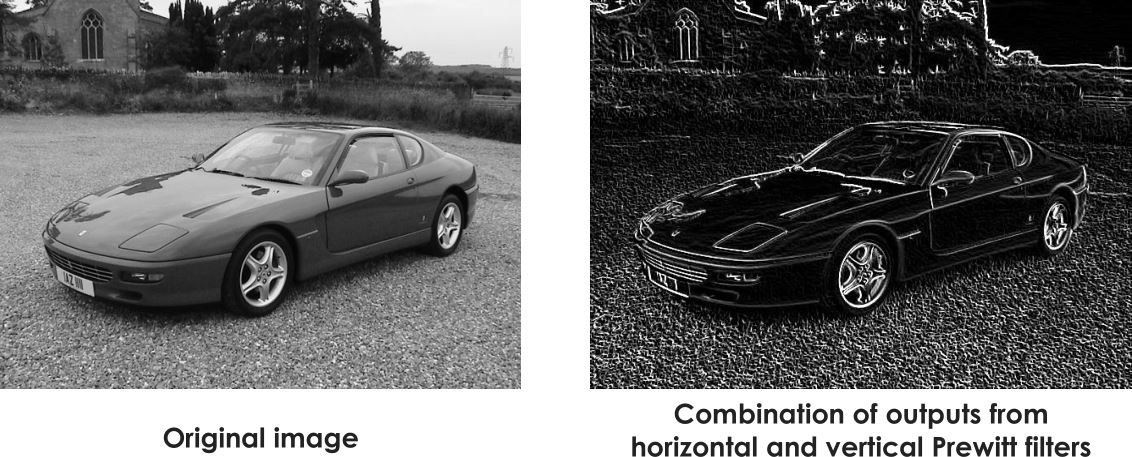
\includegraphics[height=1.75in]{prewittfilterexample}
		\caption[Prewitt filter example]{Prewitt filter example.}
		\label{fig:prewittfilterexample}
	\end{figure}

	\subsubsection{The Sobel Filter}
	\begin{bulletedlist}
		\item The Sobel filter was conceptualized by Irwin Sobel and Gary Feldman from the Stanford Artificial Intelligence Laboratory (SAIL) in the 1960s.
		\item It is similar to the Prewitt Filter, with the only change being in the central values of the positive and negative numbers, which are now +2 and -2 instead of +1 and -1.
		\item This filter can give better intensities in the regions containing edges, in comparison to the results from the Prewitt Filter.
	\end{bulletedlist}

	\begin{figure}[h]
		\centering
		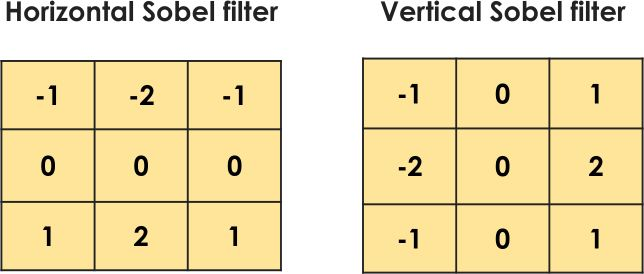
\includegraphics[height=1.0in]{sobelfilter}
		\caption[Sobel filter]{Sobel filter.}
		\label{fig:sobelfilter}
	\end{figure}
	\begin{figure}[h]
		\centering
		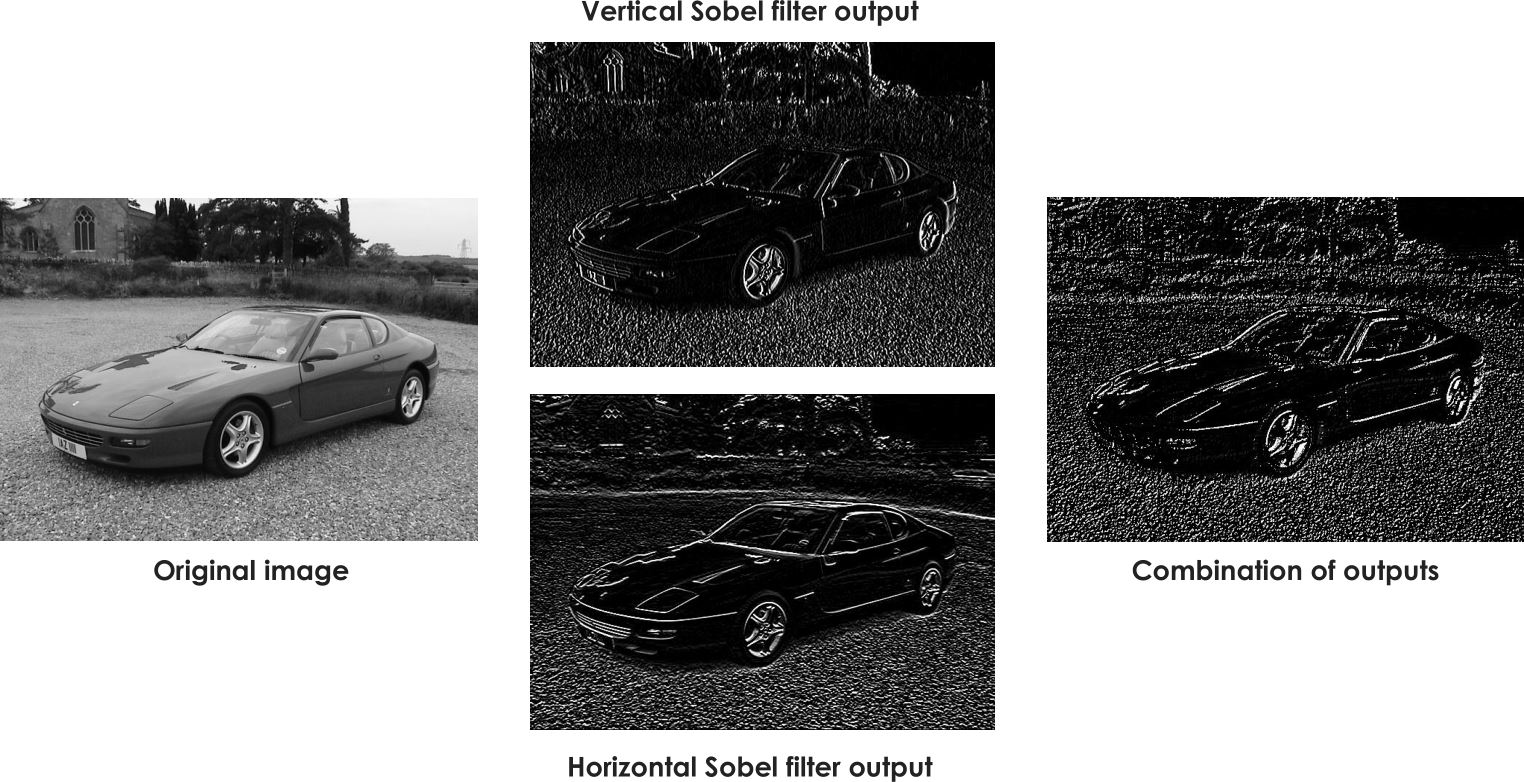
\includegraphics[height=2.5in]{sobelfilterexample}
		\caption[Sobel filter example]{Sobel filter example.}
		\label{fig:sobelfileterexample}
	\end{figure}


	\subsubsection{The Laplacian Filter}
	\begin{bulletedlist}
		\item The Laplacian filter (named after Pierre-Simon Laplace, the famous French scientist with several contributions in mathematical and statistical theory) is a second-order derivative filter that tries to highlight those regions where pixel intensities change abruptly.
		\item The implication of being a second-order filter is that unlike the Prewitt and Sobel Filters (which need a kernel in the horizontal and vertical directions each), the Laplacian filter only needs one kernel, which can detect both kinds of edges.
		\item One other thing to keep in mind is that Laplacian Filters are very sensitive to noise. So in many cases, the image may need to be smoothed out before applying the Filter.
	\end{bulletedlist}

	\begin{figure}[h]
		\centering
		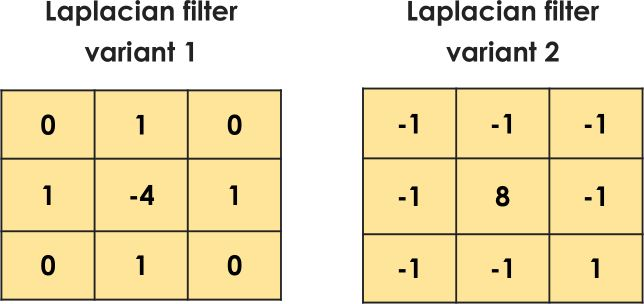
\includegraphics[height=1.0in]{laplacianfilter}
		\caption[Laplacian filter]{Laplacian filter.}
		\label{fig:laplacianfilter}
	\end{figure}
	\begin{figure}[h]
		\centering
		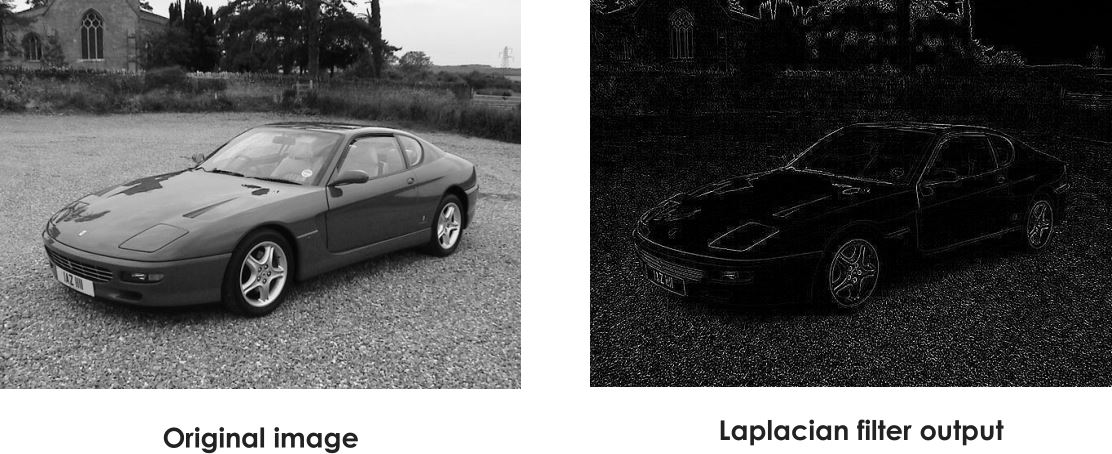
\includegraphics[height=1.75in]{laplacianfilterexample}
		\caption[Laplacian filter example]{Laplacian filter example.}
		\label{fig:laplacianfilterexample}
	\end{figure}


	\subsection{Convolution on RGB images}
	\begin{bulletedlist}
		\item When performing the convolution operation on RGB images as opposed to gray scale, the number of channels in the filter must equal the number of channels in the image (3).
		\item To compute the output of this convolution operation for example, we take the 3x3x3 filter, and first place it in the upper-left most position.
		\item Notice that the 3x3x3 filter has 27 numbers.
		\item So we take each of these 27 numbers, multiply them with the corresponding first 27 numbers (9 each - 3x3 from the red, green and blue channels), and add up those products to get a final sum.  That sum goes into the relevant cell in the output.
	\end{bulletedlist}

	\begin{figure}[h]
		\centering
		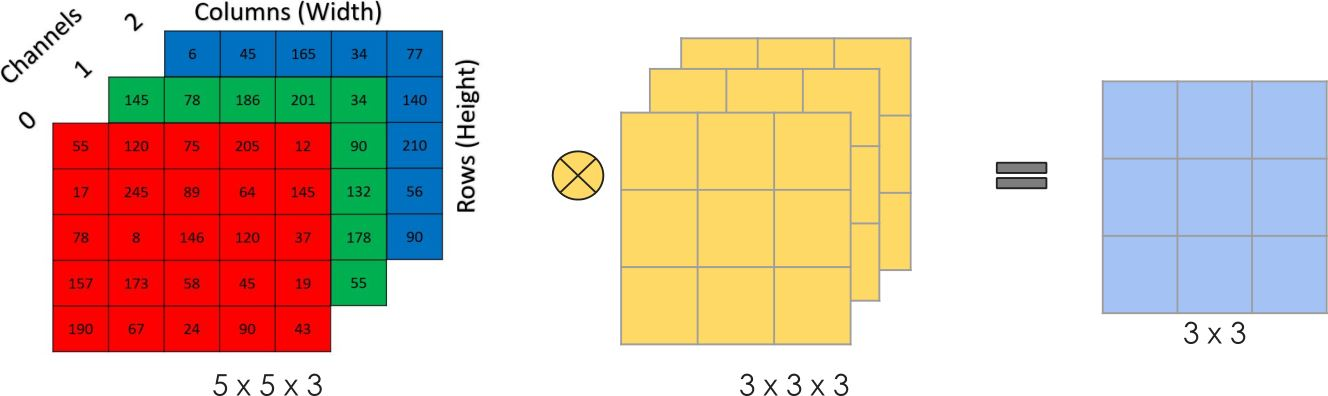
\includegraphics[height=1.35in]{convolutiononrgbimages}
		\caption[Convolution on RGB images]{Convolution on RGB images.}
		\label{fig:convolutiononrgbimages}
	\end{figure}
	\begin{figure}[h]
		\centering
		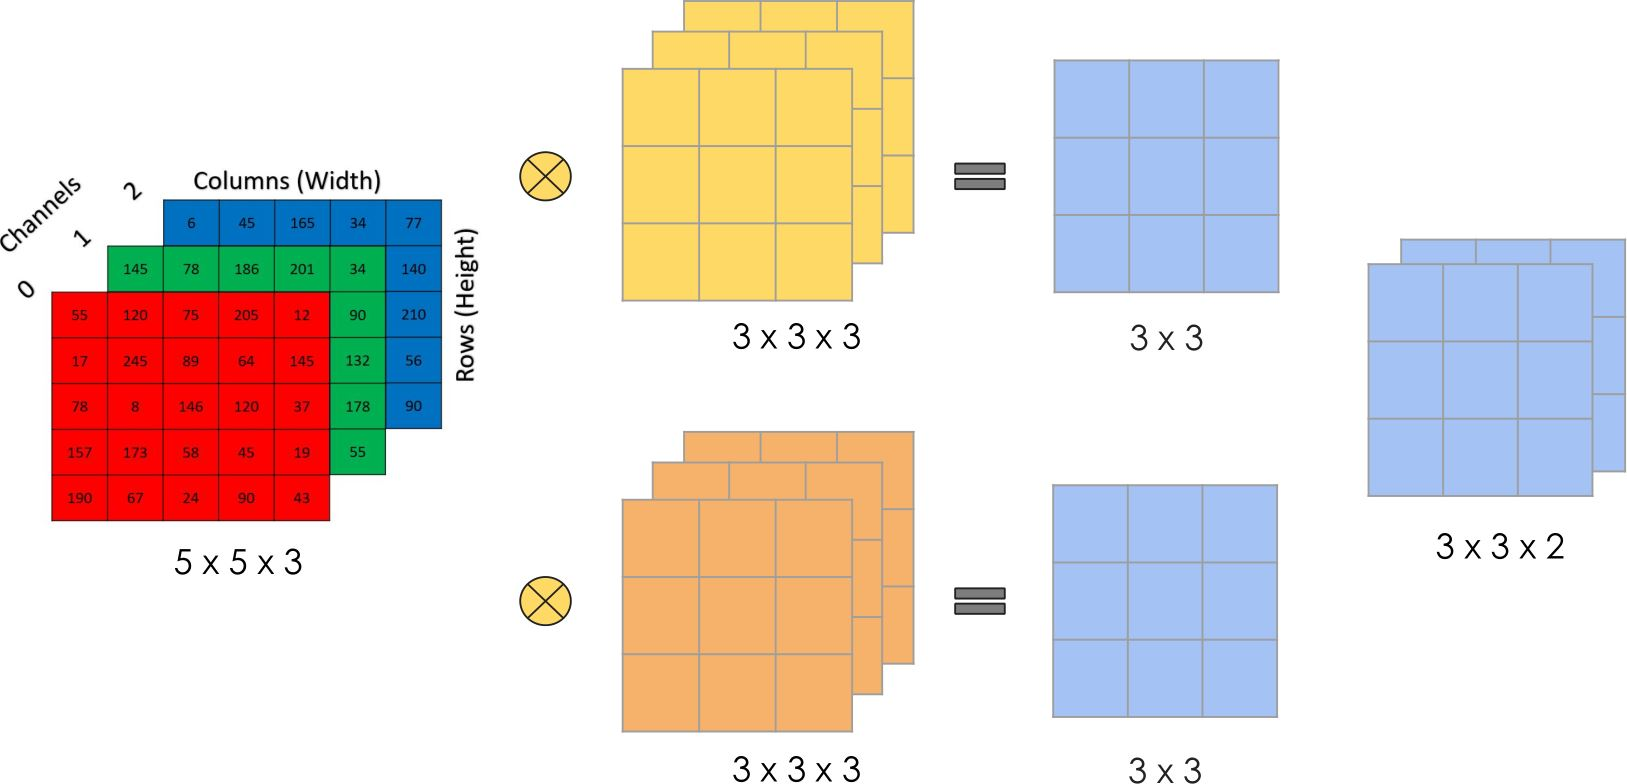
\includegraphics[height=1.75in]{convolutionwithmultiplefilters}
		\caption[Convolution with multiple filters]{Convolution with multiple filters.}
		\label{fig:convolutionwithmultiplefilters}
	\end{figure}


	\subsection{Convolutional Neural Networks (CNNs)}
	\begin{bulletedlist}
		\item However, the Computer Vision industry came to understand that such handcrafted filters would not easily generalize across all kinds of images.
		\item There are a lot of complex patterns that need to be detected in many kinds of images, and it is far from trivial to think of all the expected patterns in an image and design handcrafted filters that could try and capture all of those patterns. Such an endeavor (similar to feature engineering) is ideally something we would want to automate in some way to help the model scale and generalize well to different tasks.
		\item The idea of Convolutional Neural Networks is that while the dimensions of the convolution filters might remain a hyperparameter (which we give to the model), the values of the convolution filters themselves, could become learnable parameters. These are values which the model would learn by itself through the iterative cycle of forward propagation and back propagation, to find the filter values that work best for that predictive task.
		\item This turns out to be the magic of Convolutional Neural Networks (CNNs), and this is one of the main reasons why they have enjoyed great success in image prediction tasks across a wider variety of image-related data than was previously possible.
		\item So the way convolutional filters really work in CNNs is by the Neural Network itself learning the best values / parameters of the filter - this eliminates the need for hand-coding values and the developer having to choose good filter values for image prediction tasks.
		\item In the coming module, we will learn more about some other architectural building blocks of a CNN, before understanding their end-to-end structure and getting a sense for all the image manipulation operations happening in the various layers of the CNN.
	\end{bulletedlist}

	\begin{figure}[h]
		\centering
		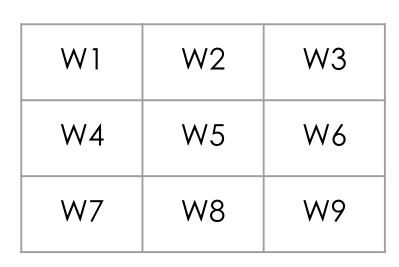
\includegraphics[height=1.0in]{convolutionneuralnetworkweights}
		\caption[Convolution weights are treated as learnable parameters]{Convolution weights are treated as learnable parameters.  Rather than us handcrafting the values of the Ws in the filter, in a CNN, we merely give the dimensions of the filter, but ask the CNN to learn the best values of Ws for the task by itself.}
		\label{fig:convolutionneuralnetworkweights}
	\end{figure}


	\subsection{Padding, Strides, and Pooling}
	\begin{bulletedlist}
		\item We have now understood the mathematical working of the Convolution operation, which is a sum of the element-wise products between the input and the filter. This is carried out through a sliding mechanism in order to generate each number in the output feature map (see \figurename{}s~\ref{fig:convolutionoperationstepsa} and~\ref{fig:convolutionoperationstepsb}).
		\item This mechanism of the vanilla Convolution Operation has three significant drawbacks:
		\item The first drawback of Convolution is that it under-utilizes pixels at the edge of the image (see \figurename~\ref{fig:convolutionunderutilizespixels}), especially the pixels at the corners, or close to the corners in relatively large images.  These pixels may only be utilized a small number of times by the sliding filter, in comparison to pixels closer to the center of the image.  For example: The 0 pixels circled in the corners would only be utilized once by the sliding filter in all its movement across the rows and columns of the image.
		\item This drawback of convolutions is a significant disadvantage for images where there is important information in the corners or edges of the image.  For example: In this cropped image of the duck, the vanilla Convolution Operation may perform poorly in classifying the image as a duck, because the crucial information about the shape of the duck's head, which is needed in classifying this image as that of a duck, is only in the corner of the image. Such regions, as we have seen, are poorly utilized by the vanilla convolution operation.
		\item The second drawback of Convolution has to do with the dimensionality of the convolution process - as we see in the example below, the 3x3 convolution filter decreases the dimensions of the image from 6x6 in the input, to 4x4 in the output.
		\item The generalized formula is that for an input (n,n) and filter size (f,f), the output feature map will have dimensions (n-f+1, n-f+1), which is a reduced size in comparison to the image input size (see~\ref{fig:convolutionoperationstep6}).
		\item The third drawback of convolution is that the convolution operation records the precise position of each of the features in the input. However, this would mean that just a small movement in the position of a feature would give us a different output.
		\item That may not always be ideal, and sometimes it may just be required to detect only the presence of an object in the image and not exactly where it is present.  In that case we do not need exact positions, but just need to validate the presence of the object in the whole image.
	\end{bulletedlist}

	\begin{figure}[h]
		\centering
		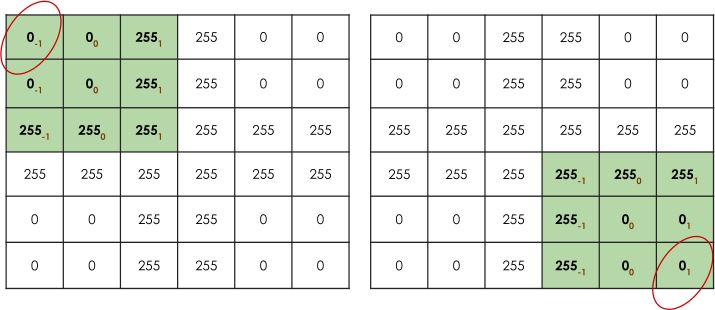
\includegraphics[height=1.1in]{convolutionunderutilizespixels}
		\caption[Convolution under utilizes edge pixels]{Convolution under utilizes edge pixels.}
		\label{fig:convolutionunderutilizespixels}
	\end{figure}

	\subsubsection{Padding}

	\begin{bulletedlist}
		\item The first two previously-mentioned drawbacks of convolutions can both be addressed through a single technique, padding.
		\item Padding is a simple trick to add extra pixels to the edges or boundaries of the image, so that the effective size of the image gets increased. This increase in effective size of the image solves both of the first two drawbacks of convolution in the following ways:
		\begin{bulletedlist}
			\item It solves the problem of under-utilized edge pixels, because now the pixels originally at the edge are closer to the center and will be utilized more often by the convolution filter.
			\item It also solves the shrinking problem of convolutions, because padding creates an enlarged image, and shrinking the enlarged size can give an output with the original size.
		\end{bulletedlist}
		\item For example, in \figurename~\ref{fig:paddingnopadding}, we observe that the input image, with a size of 4x4, shrinks to an output size of 2x2, when a 3x3 convolution filter is applied on it.
		\item The disadvantage of shrinking exhibited by the convolution operation, can be addressed using padding as shown below.  Here we pad the input image with zeros (0) along the boundaries, to effectively convert it from a 4x4 image to a 6x6 input image.  When a 3x3 filter is convolved over a 6x6 image, the output is a 4x4 matrix which is the same size as the original 4x4 input.
		\item Thus, padding effectively helps us get the same output size as the input, and avoid shrinkage.
	\end{bulletedlist}

	\begin{figure}[h]
		\centering
		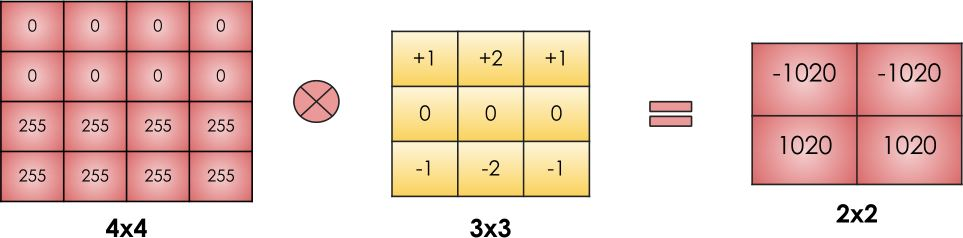
\includegraphics[height=1.1in]{paddingnopadding}
		\caption[Convolution without padding shrinks the matrix]{Convolution without padding shrinks the matrix.}
		\label{fig:paddingnopadding}
	\end{figure}
	\begin{figure}[h]
		\centering
		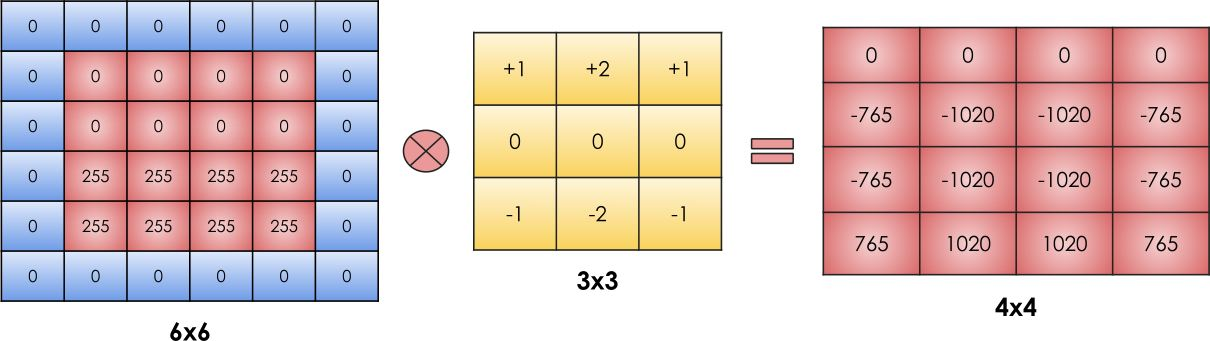
\includegraphics[height=1.25in]{paddingwithpadding}
		\caption[Using padding prevents matrix shrinking]{Using padding prevents matrix shrinking.}
		\label{fig:paddingwithpadding}
	\end{figure}

In the computer vision literature, two types of padding are described:
	\begin{bulletedlist}
		\item Valid Padding: This is the least used method as this essentially means no padding.  Here we do not perform any padding operation on the array (see \figurename~\ref{fig:validpadding}).
		\begin{bulletedlist}
			\item We observe below that the output size of the array decreases to 2x2 when a 4x4 input image is convolved using a 3x3 filter without any padding.
		\end{bulletedlist}
		\item Same Padding: It pads the input size in-order to make the output size same as the input size.  One of the basic type of same padding is called Zero Padding. In this, we add/pad zeros to all the edges of an image to prevent the loss of the original pixel values of the image.
		\begin{bulletedlist}
			\item We observe that the shape of the output is now the same as that of the input image when we apply zero padding on the input image. Thus padding helps in maintaining the output shape of the image to the same as the input even after convolution.
Padding with zeros converts the 4x4 input to 6x6 (see \figurename~\ref{fig:samepadding}).
			\item This causes the output to be 4x4, the same as the original input size.
		\end{bulletedlist}
	\end{bulletedlist}

	\begin{figure}[h]
		\centering
		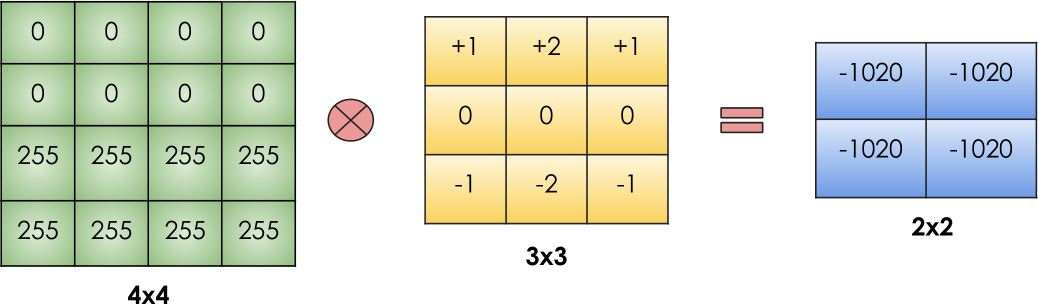
\includegraphics[height=1.1in]{validpadding}
		\caption[Valid padding]{Valid padding.}
		\label{fig:validpadding}
	\end{figure}

	\begin{figure}[h]
		\centering
		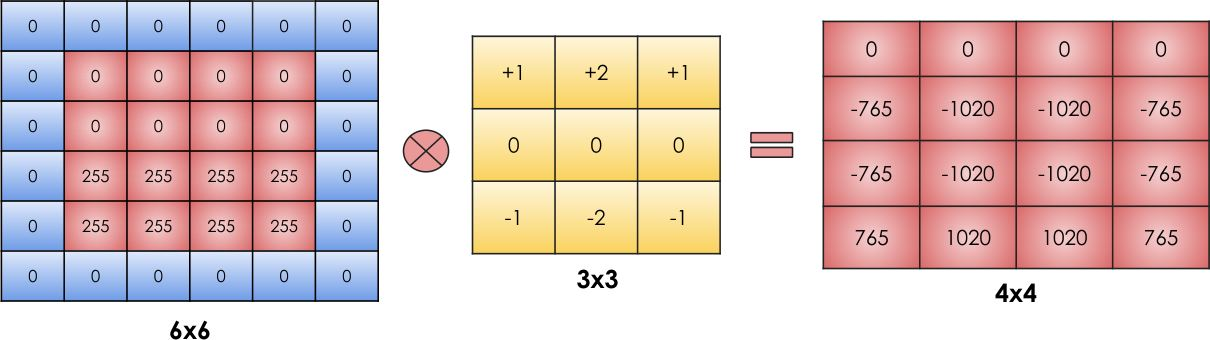
\includegraphics[height=1.1in]{samepadding}
		\caption[Same padding]{Same padding.}
		\label{fig:samepadding}
	\end{figure}


	\subsubsection{Strides}

	\begin{bulletedlist}
		\item The third drawback of convolutions, however, about the operation being too precise, may be addressed through another idea called Strides.
		\item We observe during convolution that we slide from the top-most corner to the bottom-most corner by a shift - this shift is called the Stride.
	\end{bulletedlist}

	\begin{figure}[h]
		\centering
		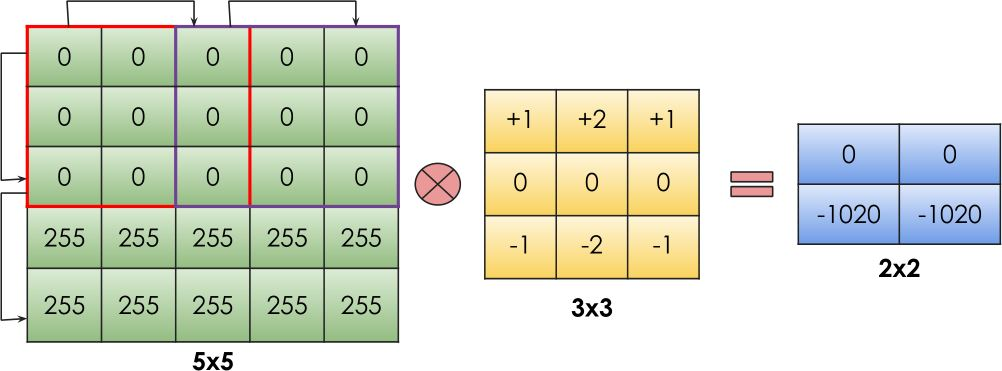
\includegraphics[height=1.25in]{strides}
		\caption[Stride]{Stride.}
		\label{fig:strides}
	\end{figure}


	\subsubsection{Mathematical Interpretation of Padding and Strides}

Let us understand the mathematical interpretation of padding and strides using some examples.

	\begin{table}
        \centering
        \caption[Padding and strides examples]{Padding and strides examples.}
        \label{tab:}
		\begin{tabular}{|p{0.5\textwidth-2\tabcolsep}|p{0.5\textwidth-2\tabcolsep}|} \hline
			\tablecolumnheadervlinesone{Example 1 - Only Padding} & \tablecolumnheadervlinestwo{Example 2 - Using Padding and Strides} \\ \hline
			Size of the input image (nxn): 4x4 \newline
Size of the filter (fxf): 3x3 \newline
Padding (p): 1 &
	        Size of input image (nxn): 5x5 \newline
Size of the filter (fxf): 3x3 \newline
Padding (p): 0 \newline
Stride (s): 2 \\ \hline
			 The shape of the output can be calculated using the formula: n+2p-f+1 \vspace{\baselineskip}\newline
So according to our example, the output shape would be: 4+(2*1)-3+1 = 4 &
	        The shape of the output can be calculated using the formula: int((n+2p-f)/s+1) \vspace{\baselineskip}\newline
So according to our example, the output shape would be: int((5+(2*0)-3)/2+1) = 2 \vspace{\baselineskip}\newline
Note: int() in Python rounds the number down to its nearest integer value. int(3.6)=3 \\ \hline
		\end{tabular}
	\end{table}

	\subsubsection{Pooling}

	\begin{bulletedlist}
		\item There is one more method that helps in eliminating the unwanted information from an image, which is more common, similar, and robust to small changes in the location of features in the input. This method is called Pooling.
		\item There are usually two common mechanisms used in pooling, max pooling and average pooling.
		\item Max pooling:
		\begin{bulletedlist}
			\item Max Pooling breaks the convolutional layer output into smaller patches. It is often, for example, a series of 2x2 pixel areas. So it is as if, in this example, there is a 2x2 filter sliding across the image with a stride of 2.
			\item Max Pooling just looks at the values in the patch and selects the maximum value from that patch. So, it helps in feature selection by removing the weak/dim features from a bright foreground and in the process, helps in down sampling or dimensionality reduction.
		\end{bulletedlist}
		\item Average pooling:
		\begin{bulletedlist}
			\item Average Pooling is exactly the same max pooling with one difference - we take the average of the values in the patch instead of the maximum value.
		\end{bulletedlist}
	\end{bulletedlist}

	\begin{figure}[h]
		\centering
		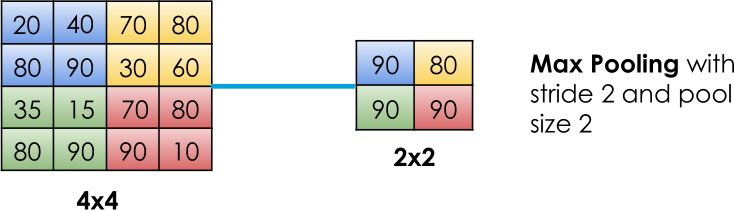
\includegraphics[height=0.85in]{maxpooling}
		\caption[Max pooling]{Max pooling.}
		\label{fig:maxpooling}
	\end{figure}

	\begin{figure}[h]
		\centering
		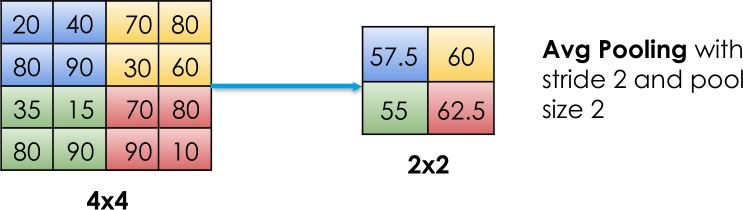
\includegraphics[height=0.85in]{averagepooling}
		\caption[Average pooling]{Average pooling.}
		\label{fig:averagepooling}
	\end{figure}

	\subsubsection{Mathematical Interpretation of Pooling}
For examples, see \tablename~\ref{tab:poolingexamples}.

	\begin{table}
        \centering
        \caption[Pooling examples]{Pooling examples.}
        \label{tab:poolingexamples}
		\begin{tabular}{|p{0.5\textwidth-2\tabcolsep}|p{0.5\textwidth-2\tabcolsep}|} \hline
			\tablecolumnheadervlinesone{Example 1 - Only Pooling} & \tablecolumnheadervlinestwo{Example 2 - Pooling with Padding and Strides} \\ \hline
			Size of the input image (nxn): 5x5 \newline
Size of the filter (fxf): 3x3 &
	        Size of input image (nxn): 5x5 \newline
Size of the filter (fxf): 3x3 \newline
Padding (p): 1 \newline
Stride (s): 2 \\ \hline
			 The shape of the output can be calculated using the formula: n-f+1 \vspace{\baselineskip}\newline
So according to our example, the output shape would be: 5-3+1= 3 &
	        The shape of the output can be calculated using the formula: int((n+2p-f)/s+1) \vspace{\baselineskip}\newline
So according to our example, the output shape would be: int((5+(2*1)-3)/2+1) = 3 \vspace{\baselineskip}\newline
Note: int() in Python rounds the number down to its nearest integer value. int(3.6)=3 \\ \hline
		\end{tabular}
	\end{table}

	\subsection{Flattening to a 1D Array}

	\begin{bulletedlist}
		\item After completing multiple iterations of the convolution and pooling operations on the image, we get feature maps of reduced dimensionality, also having multiple channels.
		\item This is a 3D Array of size (Width, Height, Channels).
		\item Since the output from the Convolution and Pooling operations is a 3D array, we can't directly use them in the fully connected layers of Neural Networks, which only accept 1D arrays of values.
		\item This is the main reason we have to flatten the output from Convolutions and Pooling into a 1D array.
		\item The number of units or values in this 3D array will be Units (U) = WxHxC
		\item Our task here is to flatten this 3D array into a 1D array of size (WxHxC, 1) = (Units, 1)
	\end{bulletedlist}

\vspace{\baselineskip}
Procedure for Flattening a 3D array:
	\begin{numberedlist}
		\item We read row-by-row for each channel starting from the first channel.
		\item Each row is appended to the 1D flattened array.
	\end{numberedlist}

\vspace{\baselineskip}
Example:
	\begin{bulletedlist}
		\item The initial size after the Convolution and Pooling Operations: 10x10x24
		\item Here we have height and width as 10, and 24 channels.
		\item Size after Flattening this 3D Matrix: (2400, 1)
	\end{bulletedlist}

	\begin{figure}[h]
		\centering
		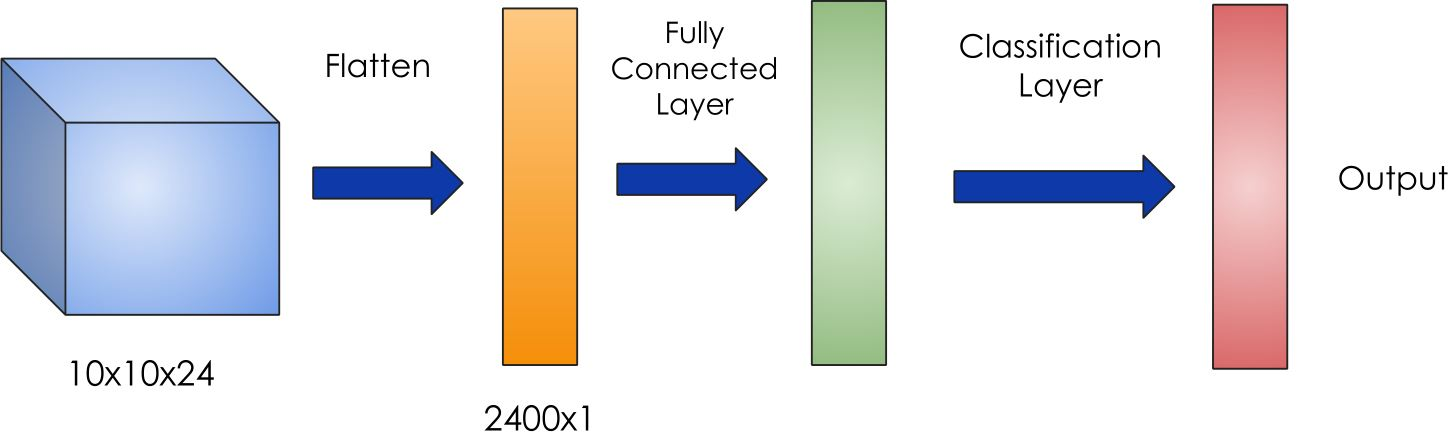
\includegraphics[height=1.2in]{flatteninganarray}
		\caption[Flattening a 3D array]{Flattening a 3D array for use in a neural network.}
		\label{fig:flatteninganarray}
	\end{figure}
